\documentclass[12pt]{article}

\usepackage{amsmath, amssymb, amsthm, graphicx, fancyhdr, textcomp, enumerate, diagbox, tcolorbox, esvect, tikz, adjustbox}


\graphicspath{{./images/}}


\usepackage{halloweenmath, tikzsymbols}

\newcommand{\R}{\mathbb{R}}
\newcommand{\Z}{\mathbb{Z}}
\newcommand{\C}{\mathbb{C}}
\newcommand{\N}{\mathbb{N}}
\newcommand{\Q}{\mathbb{Q}}
\newcommand{\Arg}{\mbox{Arg}}
\newcommand{\Log}{\mbox{Log}}
\newcommand{\conv}[1]{\mbox{conv}(#1)}

%geometry/topology
\newcommand{\bndry}{\partial}


\newcommand{\infsum}{\sum_{n = 1}^{\infty}}
\newcommand{\pf}{\fbox{proof}}
\newcommand{\cor}{\fbox{corollary}}

\theoremstyle{definition}

\newtheorem*{definition}{Definition}
\newtheorem{lemma}{Lemma}
\newtheorem{theorem}{Theorem}
\newtheorem{corollary}{Corollary}
\newtheorem{proposition}{Proposition}
\newtheorem{remark}{Remark}
\newtheorem{conjecture}{Conjecture}
\newtheorem{example}{Example}
\newtheorem{problem}{Problem}
\newtheorem{axiom}{Axiom}


\title{Modern Geometry}
\author{August}

\begin{document}

\maketitle

\section{problem 2.22}

We will construct a point set $S$ for any $n$ number of vertices which is a worst case scenario for the Scan of Grey Ham (SGH) Algorithm. Incidentally, I have already done this, only I didn't name it as such, in constructing a class of polygons with $n$ vertices which only have $1$ triangulation. "Recall" this construction. I have a truly marvelous proof, which the margins of this LaTeX document cannot contain. Luckily, I need not to write it in the margins, and will write it in the document itself. 

\begin{theorem}
Let $x_1$ be any point, and draw a line through $x_1$, call it $l$. Pick a side of $l$, and draw a curve $C$ which is concave up with respect to $l$. Now draw $n-1$ rays originating from $l$ which are all on the chosen side of $l$, ordering them by angle from one chosen direction of $l$ as $r_1,\dots, r_{n-1}$. The curve $C$ intersects the rays at points $x_1,\dots, x_{n-1}$. In this case, the Graham scan takes $2(n-1)$ steps other than ordering of the points, and this is as bad as the Graham scan can get. 
\end{theorem}

\begin{proof}
To see that this is really a worst case scenario, notice that in the Graham scan algorithm, each point contributes at most two steps. Moreover, they must have a right turn to them in order to contribute two steps. We can define a point's "contribution" to mean the number of steps which draw an edge to it. Since each step draws an edge to only one vertex, each step is contributed by a unique point. Moreover, the vertices with least angle, as well as the point $x_1$, must be connected only by left turn. Hence they only contribute one step. No matter what our first points end up being, they will always only contribute two steps. Hence the upper bound for number of steps in $2(n-1)$\\

Now we can see that every other vertex in our example contributes two steps. Since the curve is concave up, the next line is always steeper. Hence the next turn will always be a right turn, and we will always have to back up and add another step. 

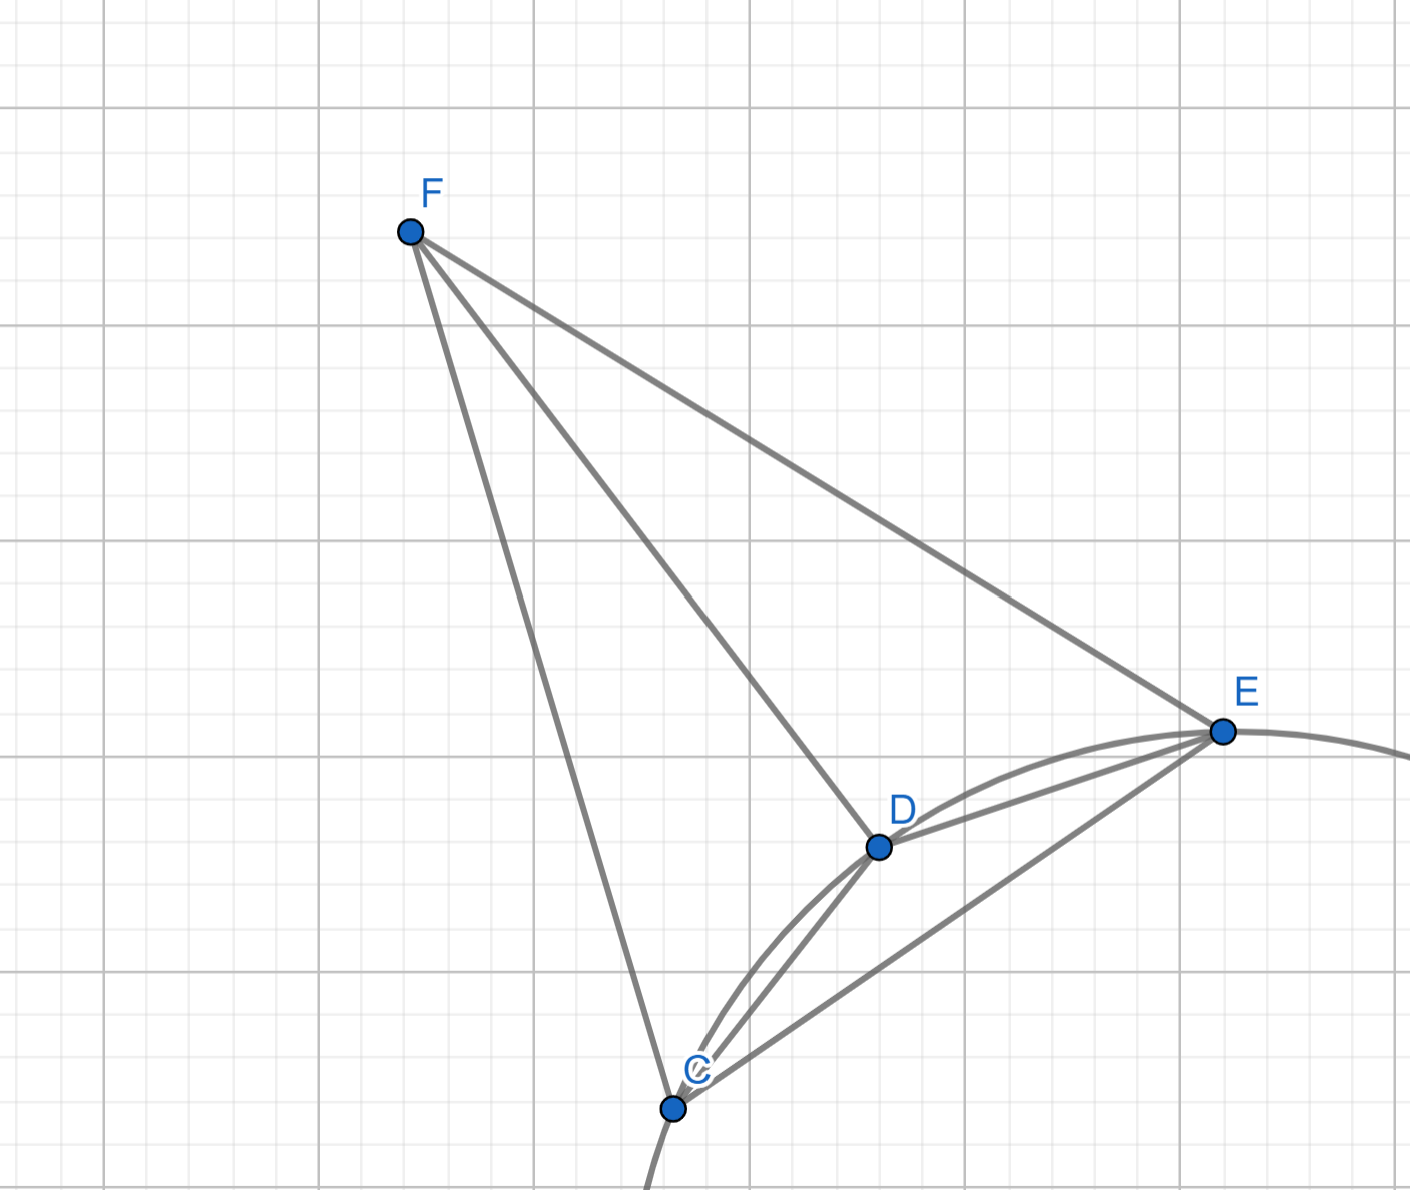
\includegraphics[scale=0.25]{concave.png} 
\end{proof}

Although this is the worst case, it doesn't really matter in the end (where the end is defined to be the order of magnitude as the number of steps increases beyond all bounds). It's still $n\log n$, and the sorting of the points is still the worst part of the algorithm.

\section{2.23}

Here I'll provide an algorithm for turning any point set $S$ into a polygon, though a simple adaptation of SGH. My original algorithm only works under the assumption that the points are in general position. I have an easy adaptation that renders this stipulation unnecessary. 

 Select a hull vertex by chosing the "least" y-value point in $S$. If there are multiple, rotate slightly that there is only one. Let $x_0$ be that point. Now draw rays from $x_0$ to the remaining points of $S$, and order the points $x_1,\dots, x_{n-1}$ by angle (the direction is immaterial). Drawing edges $x_ix_{i+1}$, labeled cyclically so that $n = 0$, is a polygon.\\

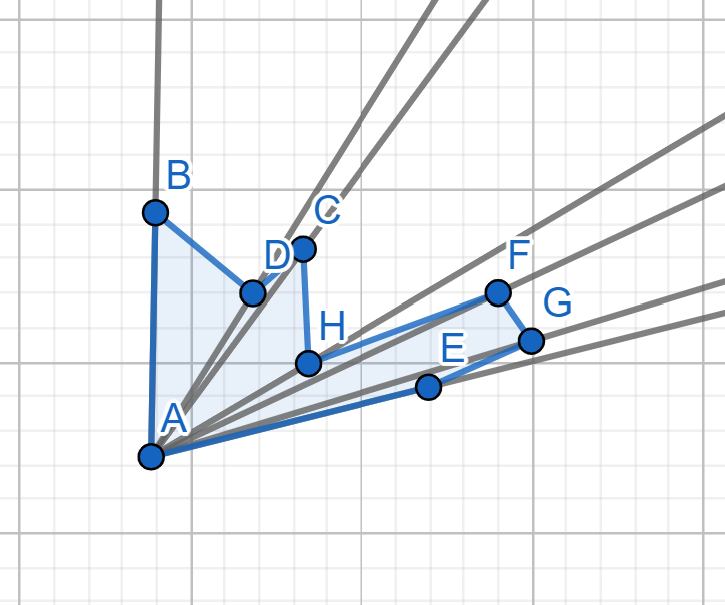
\includegraphics[scale=1]{polygon_alg.png}

To see this, it suffices to show that the edges do not cross except at their endpoints. 

Let $x_i$ and $x_j$ be distinct points. Without loss of generality, assume $i> j$. Now we consider the line segments $x_ix_{i+1}$ and $x_jx_{j+1}$, and desire to show that they do not cross (except perhaps at the endpoints). The first case is that they do in fact cross at the end-points. Then since  $x_i \ne x_j$, and since the points are in general position, it follows that they do not cross elsewhere (or else we would have three points collinear).\\

Now we suppose that $x_ix_j$ is not an edge, that is, that the difference of $i$ and $j$ is not one modulo $n$. Then there must exist some $k$ between $i$ and $j$, and a corresponding $x_i$. Without loss of generality suppose $i > j$, hence $i+ 1 \ge j$. Moreover, the line $x_1x_k$ divides the plane into two halves, and by construction of the points $x_i$ and $x_{i+1}$ as having an angle greater than that of $x_k$. Meanwhile $x_j$ and $x_{j+1}$ have angle less than or equal to that of $x_k$. Hence they lie on opposite sides of the line, and share at most the point $x_k$.\\
 Q.E.D.
 

\section{problem 2.38}

\begin{proposition}
Let $T$ be a regular tetrahedron. Let $p$ be a point not interior to it. Then the convex hull of $T$ union $p$ can have at most six faces. It is also possible have five faces (an odd number), only not if we require that $p$ be in general position with the vertices of $T$. 
\end{proposition}

\begin{proof}
First, it is easier to show that you can get an odd, so I'll start with that. Imagine the vertex $E$ which is coplanar to the face $ CBD $, as depicted in the figure. Notice that because the new plane $EBC$ formed in the convex hull, lies flat with $CBD$, it forms a new single face $BECD$. We also lose the face $BCA$, and we gain the faces $EBA$ and $ECA$. Hence in total we have added one face to the tetrahedron, and the resulting number of faces is five. This example is not in general position, but haven't yet shown that we can't do this without leaving general position. \\
 
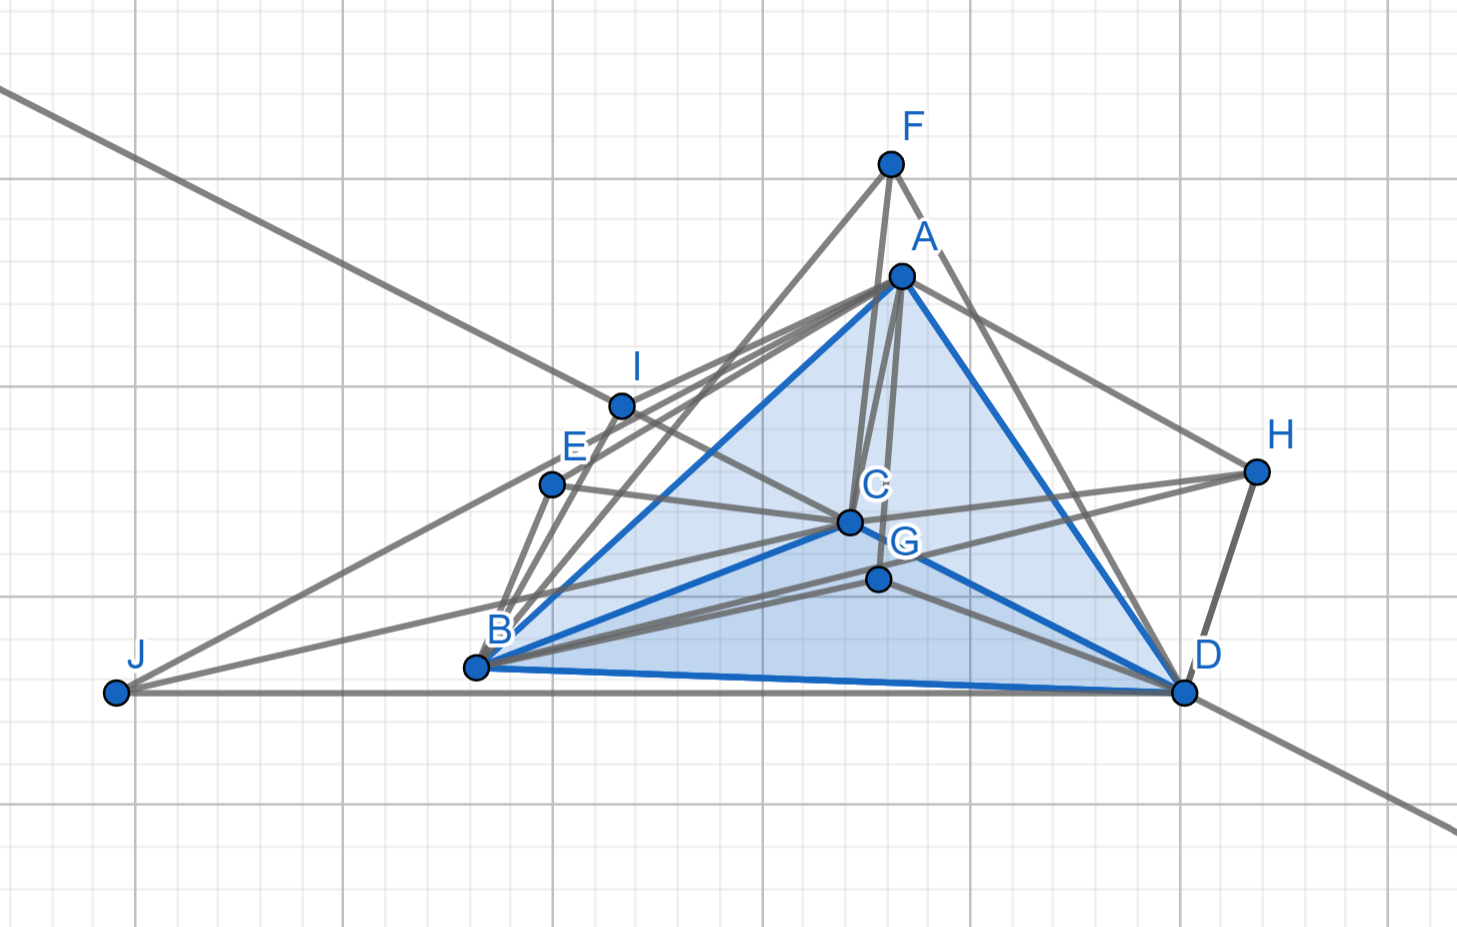
\includegraphics[scale=0.5]{bad_polyhedron_2.png} 

Now to show that six is really the best we can do. There are essentially six cases, corresponding to the points $I$, $G$, $H$, $F$, $J$ and $E$, of which the cases correspoinding to $H$ and $G$ have the greatest  number of faces. This is best argued using the symmetries of the regular tetrahedron. Notice that because the regular tetrahedron has four faces, it's faces correspond to planes, each of which divides space into two parts, one of which contains the rest of $T$.\\

Notice that if $p$ is in the interior of the region which does not contain $T$, it can see all of the face corresponding to that region. Moreover, if not in this region, the point cannot see $T$ (that is, lines from $p$ to that face cross through the boundary of $T$ other than at the face.) If we are on the tetrahedron's side of each side of the planes, then we are interior, and $p$ is not. Hence $p$ must be on the side of $p$ which does not contain $T$ for at least one of the faces. Notice also that there is, no region which is outside for each of these planes. Hence we must be on the outside for either two, three, or one of them, corresponding to $p$ being able to see two, three, or one of the faces of $T$. By the symmetry of the tetrahedron, it does not matter which of these faces can be seen; only the number of faces visible and position relative to them matters.\\

Now suppose that we can see three of the faces, but are not \textit{on} one of the planes. The $p$ can see three faces, and those faces will be covered up, forming three new faces connecting from the vertices which are visible to $p$. In total, we will have four faces in this case.\\

Now suppose that we can see two of the faces, but are not on any of the planes, as in $H$. In this case, we lose the faces $CAB$ and $BAD$, and gain the faces $BAH$, $CADH$, $BGD$, and $CHD$, it total, we have six. \\

Now suppose we lie upon two of the planes, as in $I$. This extends the tetrahedron outward, to create another tetrahedron, since it lies flat with two of the faces (since it's on the planes). Hence we have four faces in this case.\\

The rest follows pretty similarly, and we see that we always get four, five, or six faces, so six is the best we can do.\\

Notice also that in all the cases where we end up with five faces, we always lie on one of the planes. So in order to get five, we must always leave general position.

Q.E.D.


\end{proof}


\section{problem 3.10}

\begin{theorem}
The incremental algorithm fails to produce every triangulation for an arbitrary point set under rotation.
\end{theorem}
\begin{proof}
Consider the following point set: 

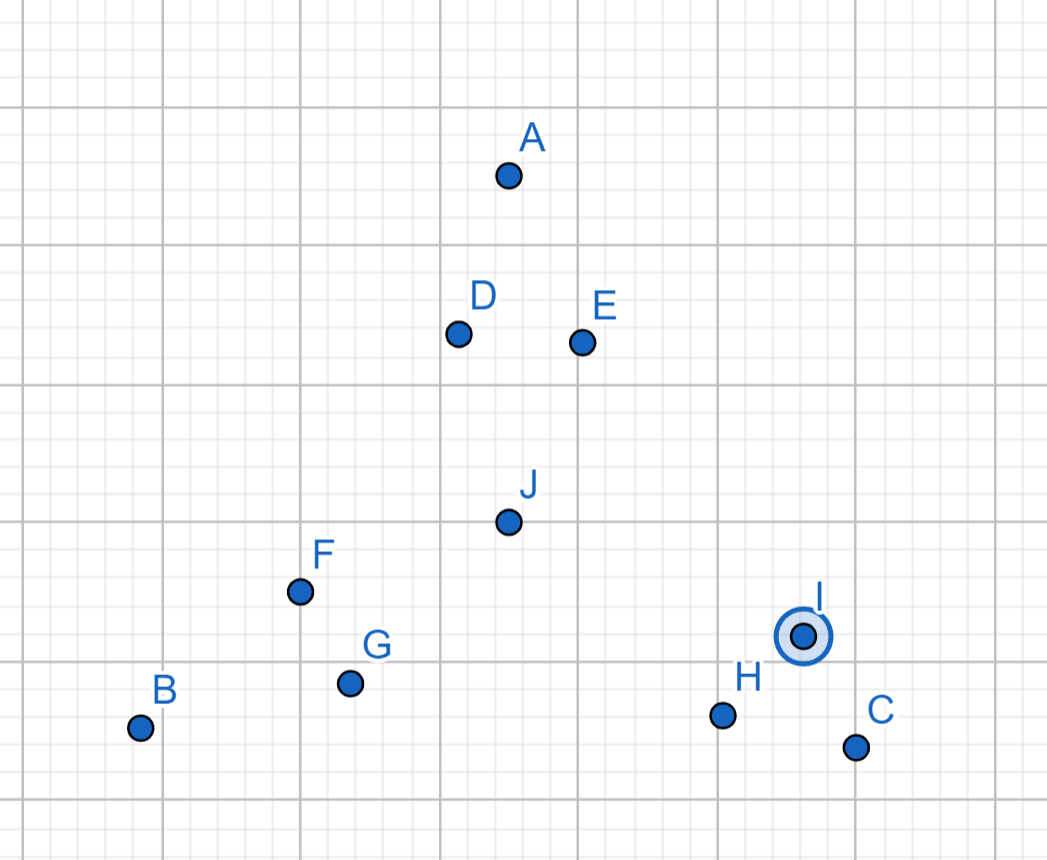
\includegraphics[scale=0.5]{point_set.png}.

Consider also the triangulation of this point set, which could be produced by the triangle splitting algorithm:
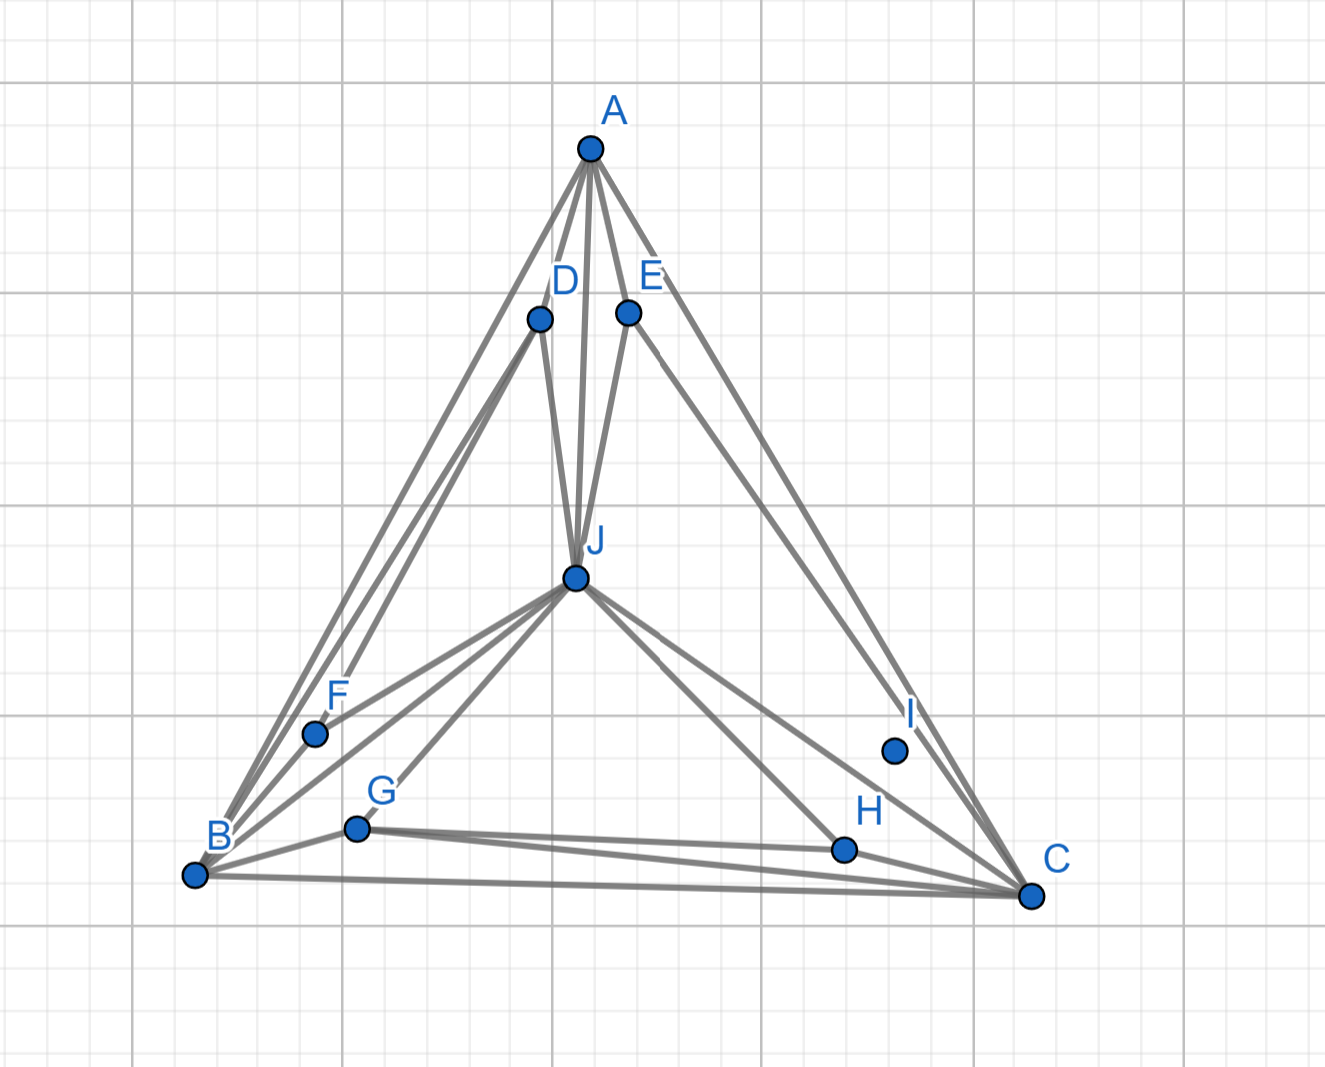
\includegraphics[scale=0.5]{counterexample.png} 

Due to the symmetry of the point set, we can chose any of the hull vertices, $A$, $B$, and $C$, without loss of generality as the "first" point after rotating, let us chose $B$. This will set the "$x$-axis" to be parallel to some tangent line, $BK$ ($K$ not in the point set) through $B$. Drawing the line $JB$, we see that there are two cases which are essentially the same: either $BK$ makes an angle with $BJ$ on the same side as $G$ or $F$. Suppose without loss of generality that it makes a greater angle on the side $F$. Now draw a line parallel to $BK$, $GL$, through the point $G$, and notice that between $BK$ and $GL$, there are no points of the point set. Therefore $G$ is "next", in this rotation for the incremental algorithm. Now notice that "second next" would be $F$. Hence we must draw the triangle $BGF$, in which case the diagonal $BJ$ cannot be drawn. But in the triangulation provided, the diagonal $BJ$ is drawn. Therefore this triangulation cannot be achieved through any rotation with the incremental algorithm. 

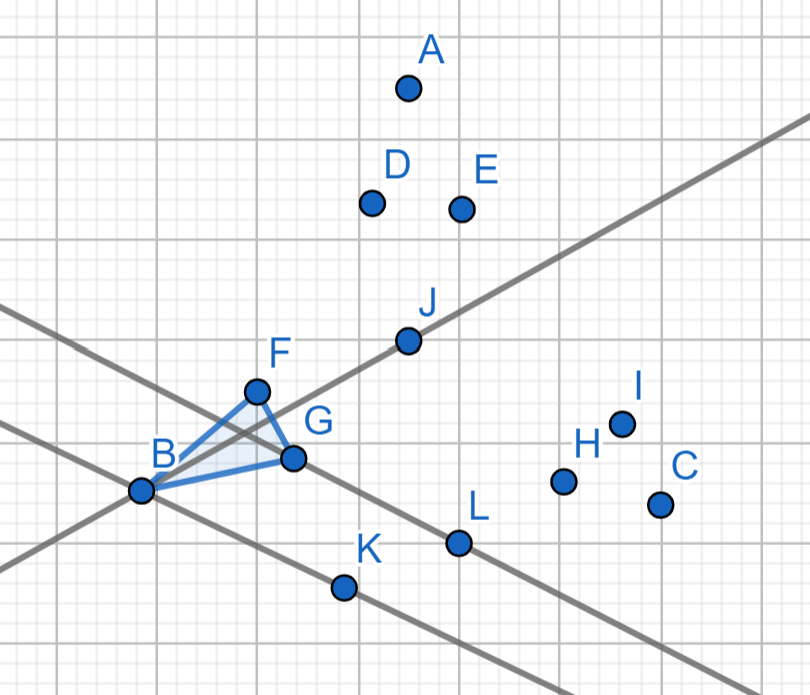
\includegraphics[scale=1]{proof_counterexample.png} 

Q.E.D.


\section{problem b}

\begin{definition}
A centerpoint of a point set $S$ in $\R^2$ is a point in $\R^2$ so that any line drawn through it must have at least two points of $S$ on both sides.
\end{definition}


\begin{lemma}
Suppose a point set $S$ contains two distinct pairs of line segments which cross, say at $x$. Then $x$ is a centerpoint.
\end{lemma}

\begin{proof}

\end{proof}

\begin{proof}
Suppose that $S$ has five vertices. Rotate the point set (or assign coordinates), so that no two points have the same $x$ or $y$ values. Draw a horizontal line $h$ which seperates the bottom two vertices and the top three. Draw a vertical line $v$ which seperates the left two points and the right three. Then $v$ and $h$ divide the plane into four quadrants, $Q_1$
\end{proof}


\end{proof}

\begin{definition}
The center of a point set $S$, denoted $C(S)$, is the set of points in $\R^2$ which are centerpoints of $S$. 
\end{definition}


I have a wild generalization that solves the assigned problem, as well as something beautiful about the set of solutions to it. I'll start with a definitition:

\begin{definition}
Let $S$ be a point set. The center of $S$, denoted $C(S)$, is the set of centerpoints to $S$. We can also define the center of a polygon to be the center of it's vertices. This is nice, because there are some amazing theorems about convex polygons that I am about to prove.
\end{definition}

\begin{theorem}
The center of a point set is always convex. 
\end{theorem}

\begin{proof}
If there are none or one point in the center, then it is clearly convex. Now suppose that there are two distinct points in the center, let them be $c_1$ and $c_2$. Let $x$ be a point on the segment between $c_1$ and $c_2$. Let $l$ be any line crossing through $x$. Now let $l_1$ and $l_2$ be the lines parallel to $l$ which cross through $c_1$ and $c_2$ respectively. $c_1$ and $c_2$ are center points, both sides of $l_1$ and $l_2$ respectively contain at least two points of $S$. Moreover, sicne $x$ is between $c_1$ and $c_2$, it follows that sides of $l$ entirely contain one side of $l_1$, and one side of $l_2$, thereby contianing the points on those sides. Threfore both sides of $l$ contain at least two points of $S$. But $l$ was just any line passing through $x$. Therefore $x$ is a center-point, for any line which crosses through it has sides which contain at least two points of $l$. Moreover, $x$ was arbitrary between arbitrary center points $c_1$ and $c_2$. Hence all points on line segments between center points are also center points. Hence the center is convex.
\end{proof}

\begin{proposition}
The center of a triangle is empty. Moreover, it is obvious that the center of a point set with fewer than three elements is also empty.
\end{proposition}

\begin{proof}
For the triangle case, notice that any line segment through an interior point crosses the triangle at two edges. The point shared by those edges is the sole vertex of the triangle which lies on it's side of the line. The cases with fewer than $3$ vertices are trivial. Note however that should three points be colinear, the between point is technically part of the center.
\end{proof}

\begin{lemma}
The center of a convex quadrilateral is a single point.
\end{lemma}

\begin{proof}
Select a pairs of edges not adjacent to each other. Then the two diagonal edges cross each other. Now consider any line which crosses through this point. Clearly both sides contain half of both of the segments on which $x$ lies (including their points), hence both sides contain twovertices of the quadrilateral. And now consider any point $p$ other than this point. Because two non-parallel lines meet at exactly one point, $p\ne x$. Now chose $l$ a line parallel to one of the diagonals, which does crosses through $p$. This line only contains the corner of the quadrilateral, hence $x$ is not a center point. Hence the center of any quadrilateral is just the set containing the point $x$ where the diagonals meet.\\


Q.E.D.
\end{proof}


\begin{lemma}
Given five points on the plane, it is always possible to select two distinct pairs of them such that the line segments between them cross. Equivalently, it is always possible to form a convex quadrilateral out of five points.
\end{lemma}

\begin{proof}
For this problem, we can assume general position. For assume that three of the points are colinear. Select the one in between, and draw a segment to any other point in the point set. This makes the lines cross at the between vertex.\\

Since we are now in general position, there are three possibilities for the shape of a convex hull: convex pentagon, convex quadrilateral, and the triangle. The convex pentagon and the quadrilateral are easy to see. The convex pentagon contains a convex quadrilateral after removing an ear. Furthermore, the quadrilateral's vertices, when chosen non-adjacent, have segments which cross.\\

This leaves us with the triangle with two interior points, call them $p_1$ and $p_2$. Since $p_1$ and $p_2$ are not colinear with any vertex of the triangle (by assumption of general position), it follows that the line $p_1p_2$ crosses the triangle which contains them at two distinct edges. The $e$ be the other edge which this line does not cross. Drawing segments from vertex of $e$ closest to $p_1$ to $p_1$, similarly for $p_2$, and including the segments $e$ and $p_1p_2$ gives us a convex quadrilateral. The non-adjacent vertices of this quadrilateral form distinct line segments which do not cross each other.\\

Having exhausted all cases, it is now apparent that the lemma holds.

Q.E.D.
\end{proof}



\begin{lemma}
Centers respect subsets. That is, if point sets $S' \subset S$, $C(S')\subset C(S) $
\end{lemma}

\begin{lemma}
Though cute, this is actually obvious. After all, if a line's sides contains at least three points of a subset, it certainly has that many points in the bigger set. This really ain't all that interesting come to think of it.
\end{lemma}


\begin{theorem}
The center of a convex $n$-gon $P$ is a convex $n$-gon for all $n>4$.
\end{theorem}

\begin{proof}
We have already seen that the center is convex. It remains to show that it is an $n$-gon. Suppose that the $n$-gon is labeled cyclically as $p_1\dots p_n$. Draw lines $p_ip_{i+2}$. These lines cross each other at $n$-points, and form a convex $n$-gon, where each crossing occurs between lines $p_ip_{i+2}$ and $p_{i+1}p_{i+3}$, and we shall call this crossing $c_i$. Notice that $Q_i = p_i\dots p_{i+3}$ forms a convex quadrilateral wose diagonals cross at $c_i$. Hence $c_i$ is a center point of the quadrilateral $Q_i$. Since the quadrilateral's vertices form a subset of the vertices of $P$, it follows by the cute yet slightly lame lemma that $c_i$ is also a center point of $P$. Hence all $c_i$ are center points. 
\\

Since the center point is always convex, it follows that the convex polygon $P'= c_1\dots c_n$ is contained within $C(P)$ (that is, that $P'\subset C(P)$). It remains to show that $C(P) \subset P'$. We proceed by contrapositive.\\

For suppose that $p$ is a point not in $P'$. Let $x$ be a point inside $P'$. Then $px$ crosses $P'$ (and only once by convexness) at an edge, call say $c_ic_{i+1}$. Let $l$ be the line crossing through $p$ which is parallel to $c_ic_{i+1}$. Since parallel lines do not cross, $l$ cannot cross through $p_{i}$ or $p_{i+2}$. Hence the side of $l$ containing $p_{i+1}$ must only contain $p_{i+1}$. Hence $p$ is not a point of $C(P)$. Hence $C(P)\subset P'$.\\

Clearly then $C(P) = P'$, a convex $n$-gon. Hence the center of a convex $n$-gon is a convex $n$-gon.  

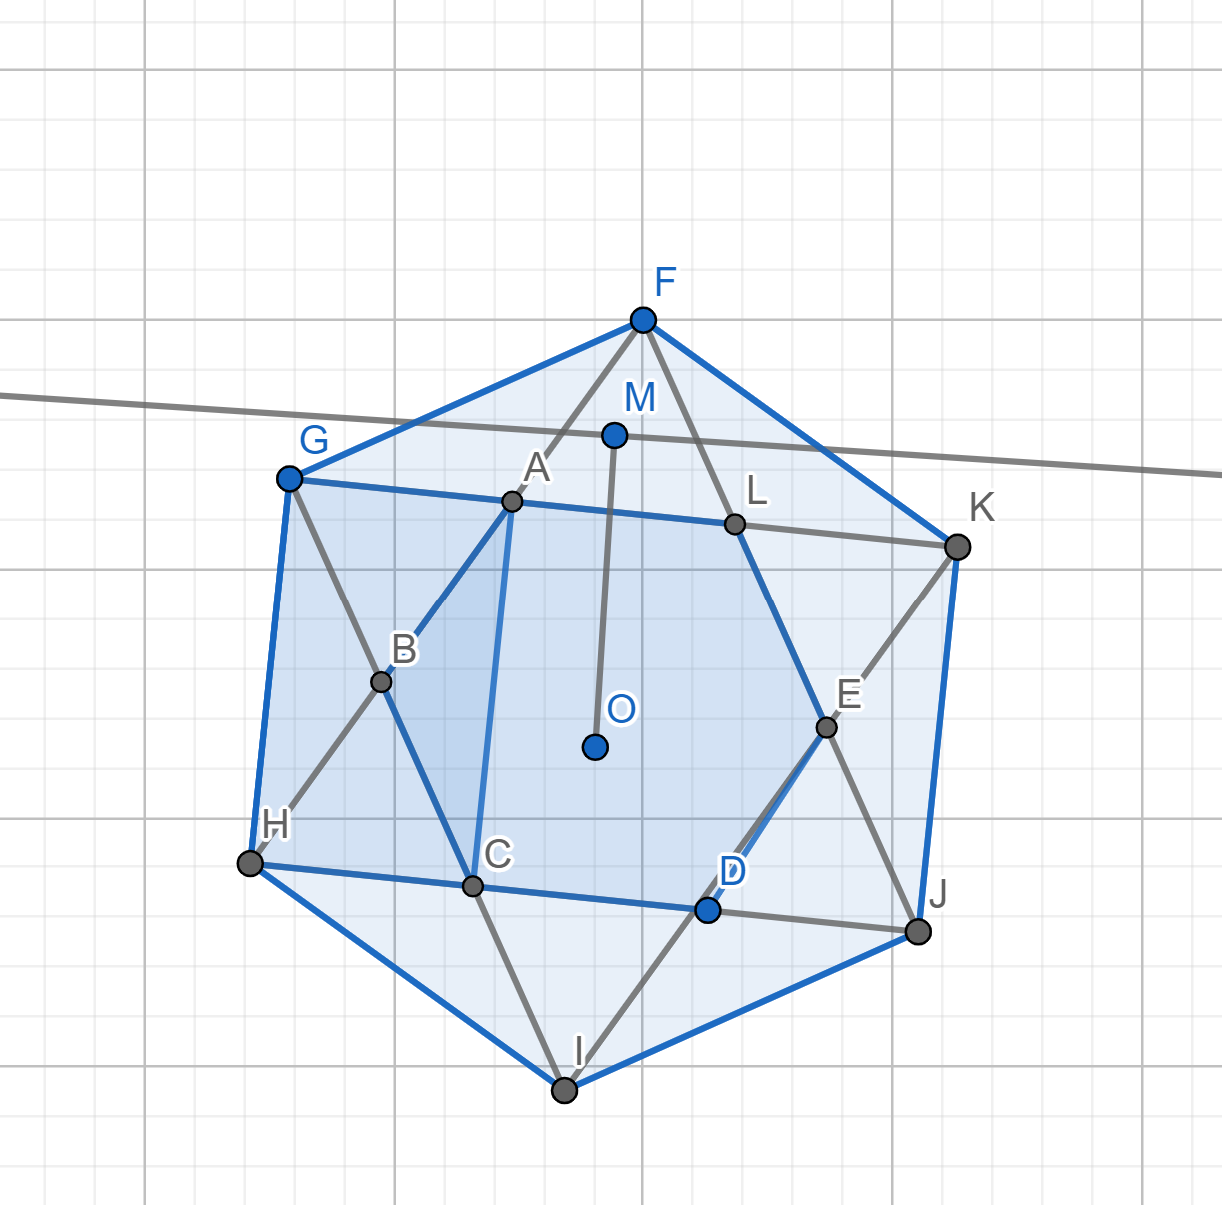
\includegraphics[scale=0.5]{center-ngon.png} 


\end{proof}

\begin{remark}
I really like this theorem.
\end{remark}

\begin{corollary}
The center of an $n$-gon with $h$ convex vertices is contained within a $h$-gon for $h>4$.
\end{corollary}


Since I might as well milk the generalization as much as possible, I have one last theorem, which is not all that interesting. 

\begin{theorem}

Suppose a point cloud $S$ has five vertices and a triangular convex hull. Then then $C(S)$ is the line segment between the two center points.
\end{theorem}

\begin{proof}

The proof is easy. Notice that either of the interior points are central. For if we draw any line through them, the line must cross some edge of the triangle $\conv{S}$, hence either side contains one of the edge vertices, as well as the point it crosses through, so each interior point is central. As a result, each of the points on the line segment 

\end{proof}

There are a few possible generalizations. One is trippy, though debateably not all that interesting. One I think would be hopeless to prove anything about. The other I doubt would be much different.


Allow me to describe my first generalization. It has two possible directions. For the purposes of this generalization, a single point, a line, and the emptyset are polygons. Once again, the center of a polygon is defined as the center of the point set formed by each of it's vertices.

\begin{definition}
The generous second center of a point set is the center of the point set union the vertices. The strict second center is the center of the center. These definitions can be carried on to any number of iterations inductively.
\end{definition}

\begin{proposition}
Let $n>4$. Then the $n$-th strict second center of a convex $n$-gon is again a convex $n$-gon.
\end{proposition}

\begin{proof}
This is obvious, and follows immediately using induction. It is cute, however.
\end{proof}

Sadly, I am now doubting that there is any interesting structure that this generalization would capture.


My second generalization would be to say that there has to be at least $n$ points on either side of a line. I doubt there would be much hope in proving this.

The other generalization would be to extend to higher dimensions. For example, in three dimensions, the center of a point set would be the set of points such that any plane passing through it would contain at least two points on both sides. I think that the cube would have a unique point in the center, and that the tetrahedron would have an empty center. I conjecture that the dodecahedron has 


\section{Problem (a)}

Find an algorithm to find the orthogonal convex hull of an orthogonal polygon.


Input a list of points $P$ listing written in cyclic order $v_1,\dots, v_n$.

\begin{itemize}
\item Loop through each of the vertices, $v_i$.
\item  Let $l$ be an empty list.
\begin{itemize}
\item Loop through each vertex not $v_i$, $v_j$. 
\begin{itemize}
\item If $v_{j+1}$ is not $i$, see if the ray $v_iv_{i+1}$ intersects the line segment $v_jv_{j+1}$. \item If they do intersect intersect, check to see if it is collinear. 
\item If they are collinear, append the closer of $v_j$ and $v_{j+1}$ to the list $l$, along with its index, in the tuple $(v_j, j)$.
\item If they are not collinear, append the intersection point to the list $l$ with the index $j$ in the tuple $(v, j)$.
\end{itemize}
\item If $l$ is empty, then pass to the next $v_{i+1}$ in the loop.

\item Now let $v$ be the closest point in $l$ to $v_i$, and le $m$ be the index corresponding to it.
\item Now re-label $v_{m+1},\dots, v_n$ as $v_{m+2},\dots, v_{n - m + i}$, and let $v = v_{m+1}$. Now update $P$ as $P = v_1\dots v_{m+1} \dots v_{n-m + i} $. (Yes, we are updating the list as we loop through it, and that is allowed in python). 
\end{itemize}
\item Now reverse the orientation for $P$, as it has been updated, and run the program again.
\end{itemize}

The time complexity of this algorithm is quadratic ($O(n^2)$), because we are looping through the number of inputs approximately twice. It actually doesn't matter that we are on occasion subtracting the number of steps, for this doesn't actually change the time complexity. So long as we have two nested loops whose lengths increase linearly with $n$, we have $n^2$.




\end{document}
